\documentclass[]{book}
\usepackage{lmodern}
\usepackage{amssymb,amsmath}
\usepackage{ifxetex,ifluatex}
\usepackage{fixltx2e} % provides \textsubscript
\ifnum 0\ifxetex 1\fi\ifluatex 1\fi=0 % if pdftex
  \usepackage[T1]{fontenc}
  \usepackage[utf8]{inputenc}
\else % if luatex or xelatex
  \ifxetex
    \usepackage{mathspec}
  \else
    \usepackage{fontspec}
  \fi
  \defaultfontfeatures{Ligatures=TeX,Scale=MatchLowercase}
\fi
% use upquote if available, for straight quotes in verbatim environments
\IfFileExists{upquote.sty}{\usepackage{upquote}}{}
% use microtype if available
\IfFileExists{microtype.sty}{%
\usepackage{microtype}
\UseMicrotypeSet[protrusion]{basicmath} % disable protrusion for tt fonts
}{}
\usepackage[margin=1in]{geometry}
\usepackage{hyperref}
\hypersetup{unicode=true,
            pdftitle={Cassy's Book},
            pdfauthor={Cassy Rivera},
            pdfborder={0 0 0},
            breaklinks=true}
\urlstyle{same}  % don't use monospace font for urls
\usepackage{natbib}
\bibliographystyle{apalike}
\usepackage{longtable,booktabs}
\usepackage{graphicx,grffile}
\makeatletter
\def\maxwidth{\ifdim\Gin@nat@width>\linewidth\linewidth\else\Gin@nat@width\fi}
\def\maxheight{\ifdim\Gin@nat@height>\textheight\textheight\else\Gin@nat@height\fi}
\makeatother
% Scale images if necessary, so that they will not overflow the page
% margins by default, and it is still possible to overwrite the defaults
% using explicit options in \includegraphics[width, height, ...]{}
\setkeys{Gin}{width=\maxwidth,height=\maxheight,keepaspectratio}
\IfFileExists{parskip.sty}{%
\usepackage{parskip}
}{% else
\setlength{\parindent}{0pt}
\setlength{\parskip}{6pt plus 2pt minus 1pt}
}
\setlength{\emergencystretch}{3em}  % prevent overfull lines
\providecommand{\tightlist}{%
  \setlength{\itemsep}{0pt}\setlength{\parskip}{0pt}}
\setcounter{secnumdepth}{5}
% Redefines (sub)paragraphs to behave more like sections
\ifx\paragraph\undefined\else
\let\oldparagraph\paragraph
\renewcommand{\paragraph}[1]{\oldparagraph{#1}\mbox{}}
\fi
\ifx\subparagraph\undefined\else
\let\oldsubparagraph\subparagraph
\renewcommand{\subparagraph}[1]{\oldsubparagraph{#1}\mbox{}}
\fi

%%% Use protect on footnotes to avoid problems with footnotes in titles
\let\rmarkdownfootnote\footnote%
\def\footnote{\protect\rmarkdownfootnote}

%%% Change title format to be more compact
\usepackage{titling}

% Create subtitle command for use in maketitle
\newcommand{\subtitle}[1]{
  \posttitle{
    \begin{center}\large#1\end{center}
    }
}

\setlength{\droptitle}{-2em}

  \title{Cassy's Book}
    \pretitle{\vspace{\droptitle}\centering\huge}
  \posttitle{\par}
    \author{Cassy Rivera}
    \preauthor{\centering\large\emph}
  \postauthor{\par}
      \predate{\centering\large\emph}
  \postdate{\par}
    \date{2019-01-16}

\usepackage{booktabs}

\begin{document}
\maketitle

{
\setcounter{tocdepth}{1}
\tableofcontents
}
\chapter{About Author}\label{about-author}

This is the start of my cook book. \textbf{Enjoy!}.

\chapter{Keto No-Fry Buffalo Cauliflower}\label{intro}

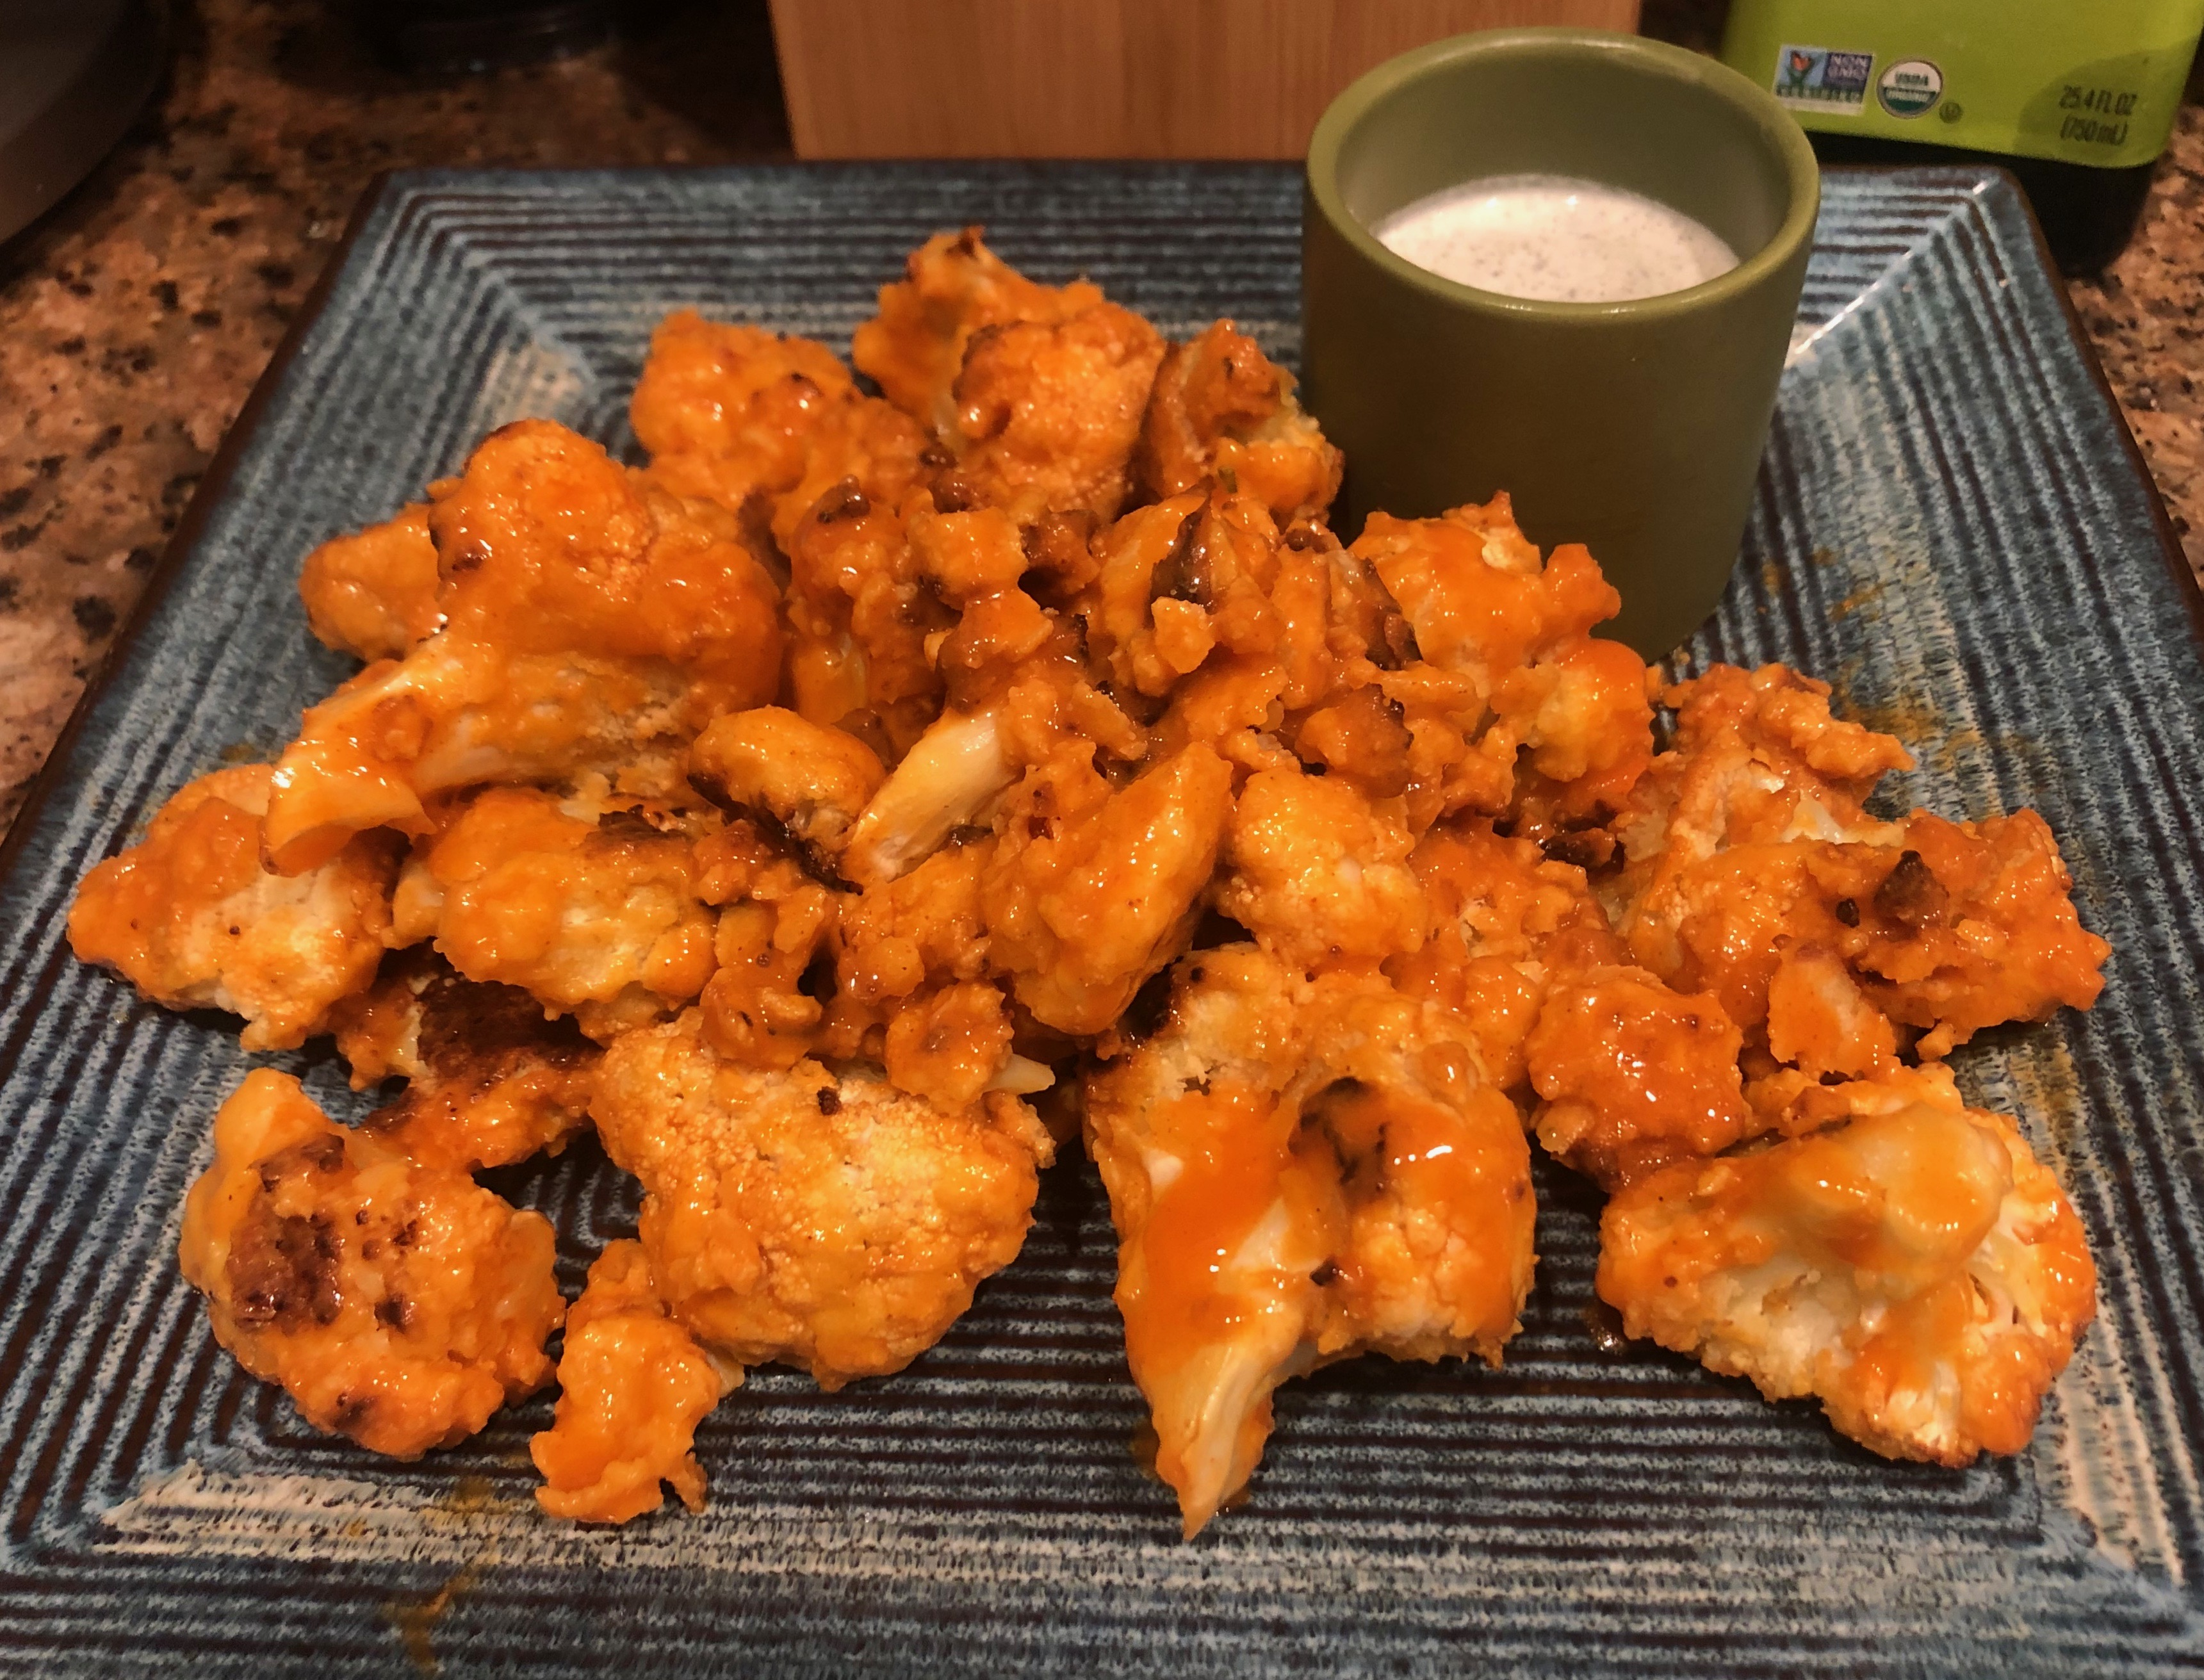
\includegraphics{../food.jpeg} 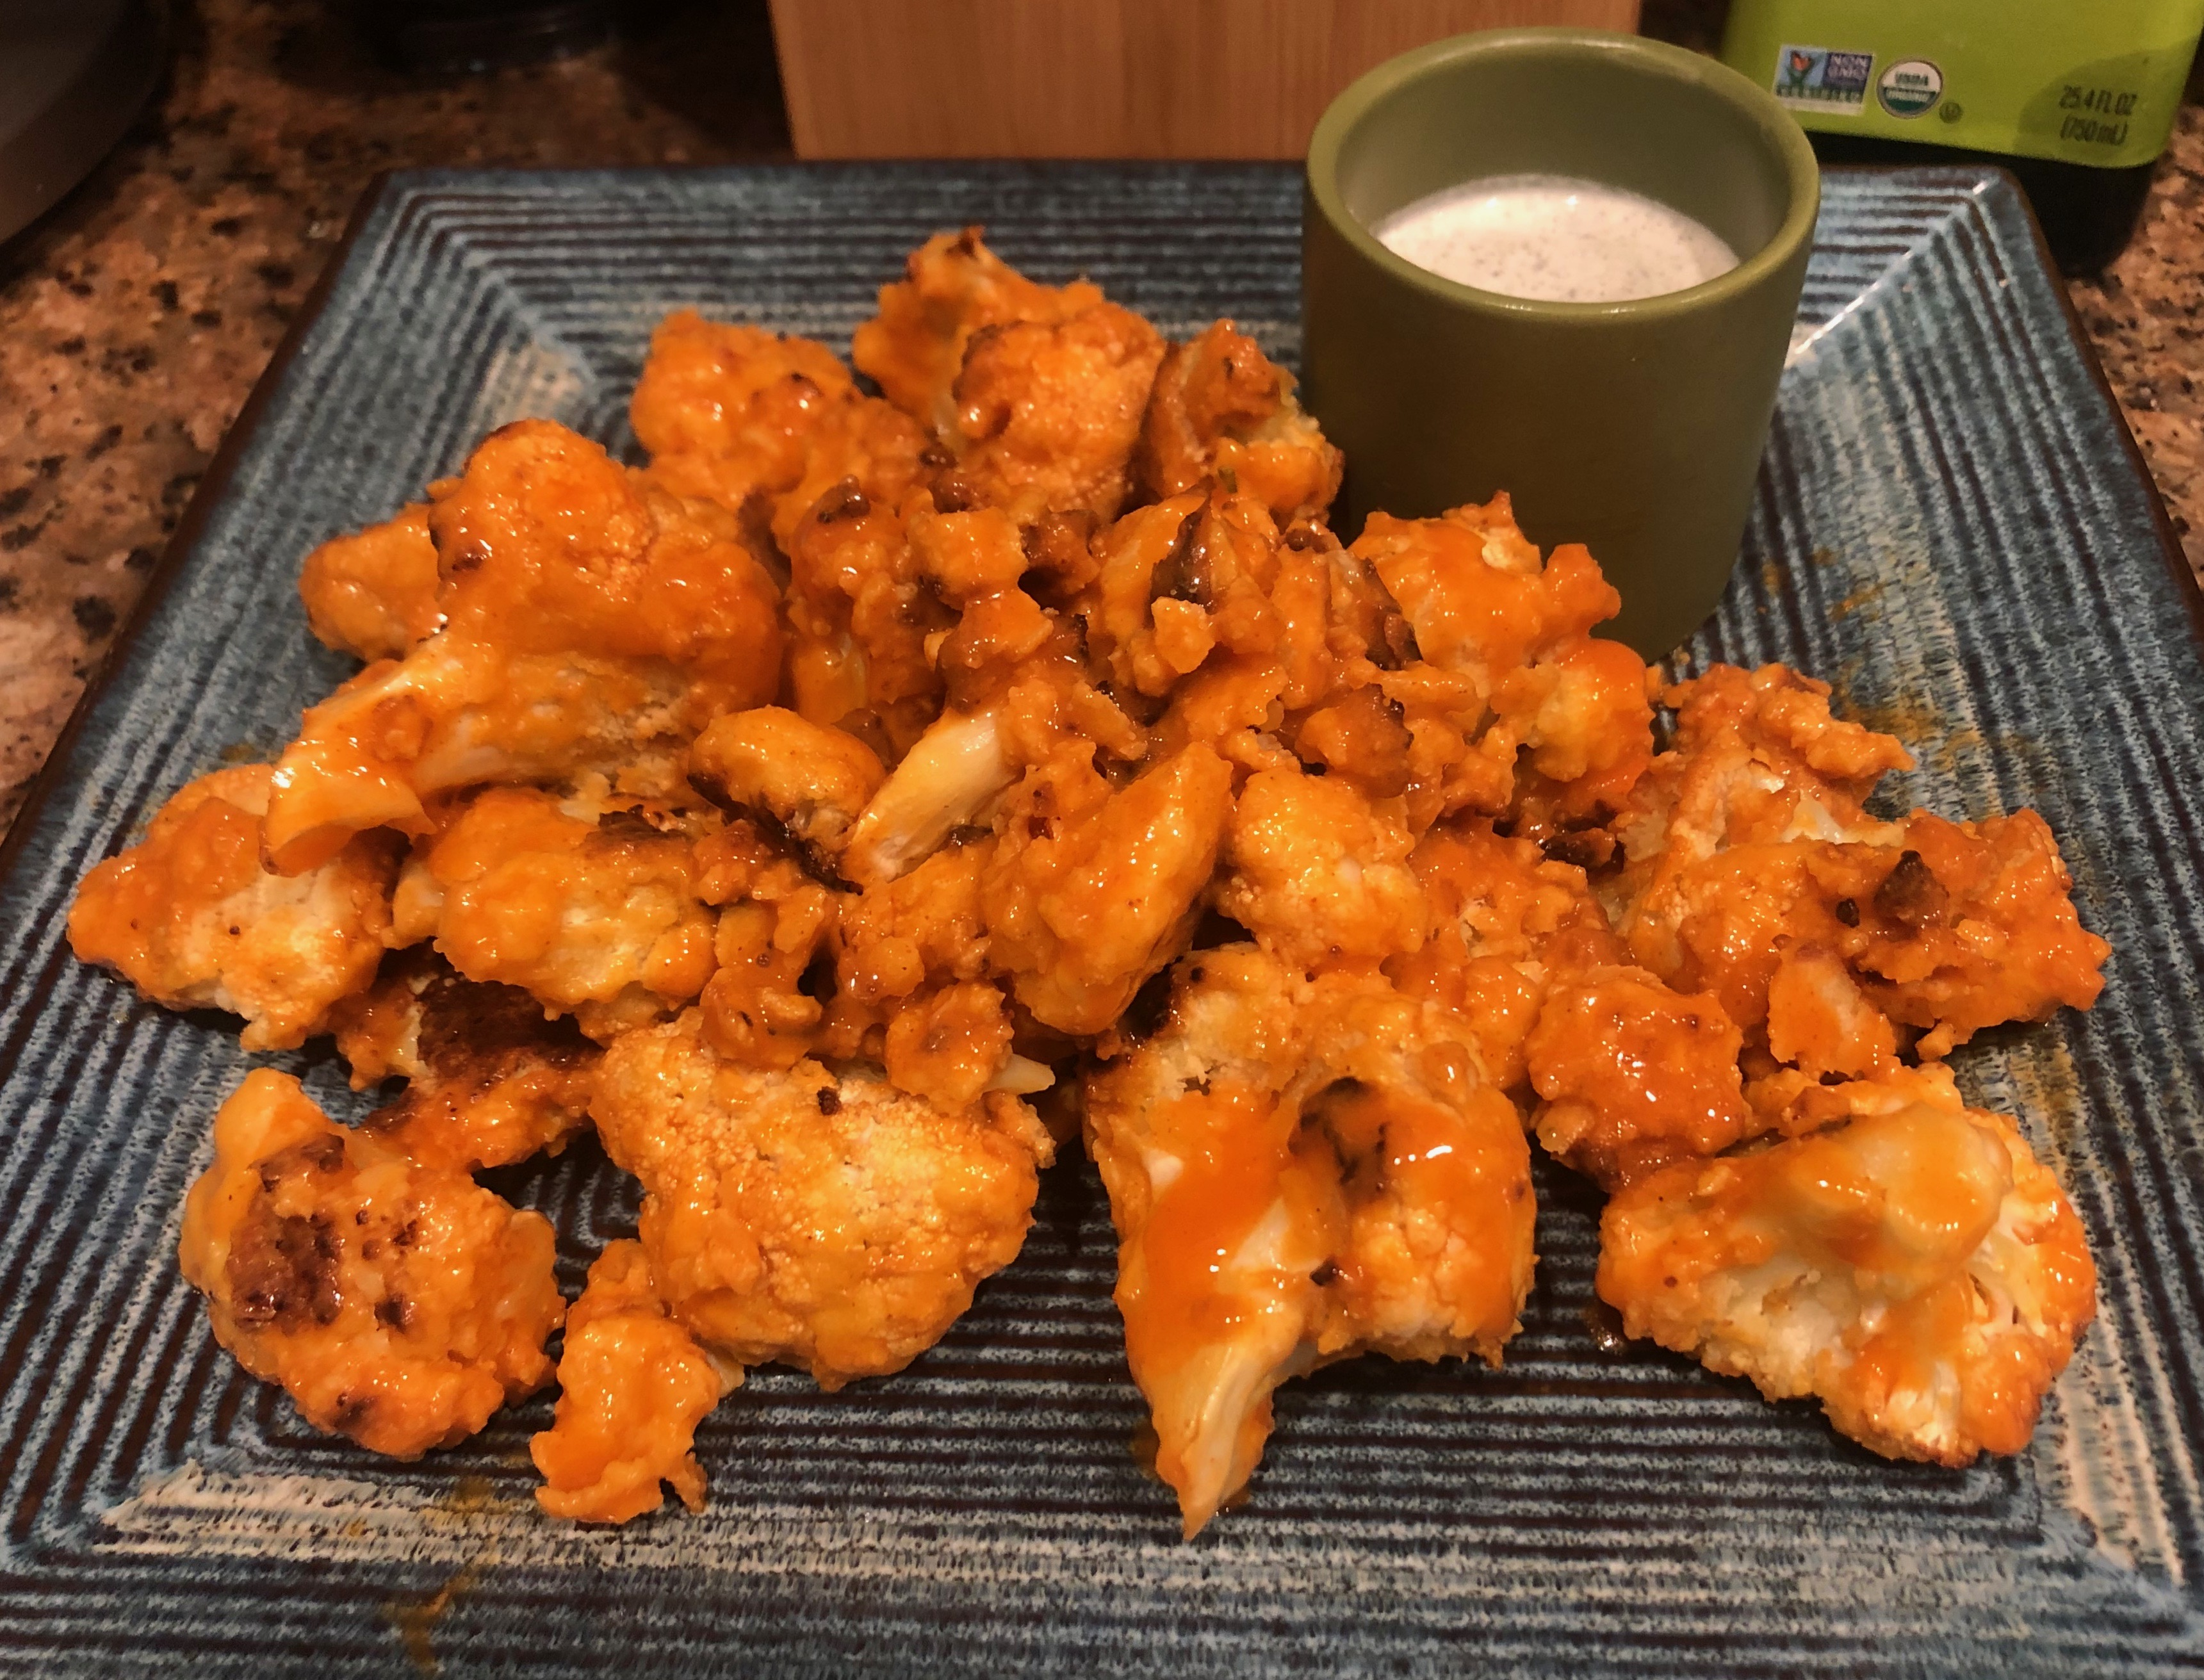
\includegraphics{../food.jpeg}
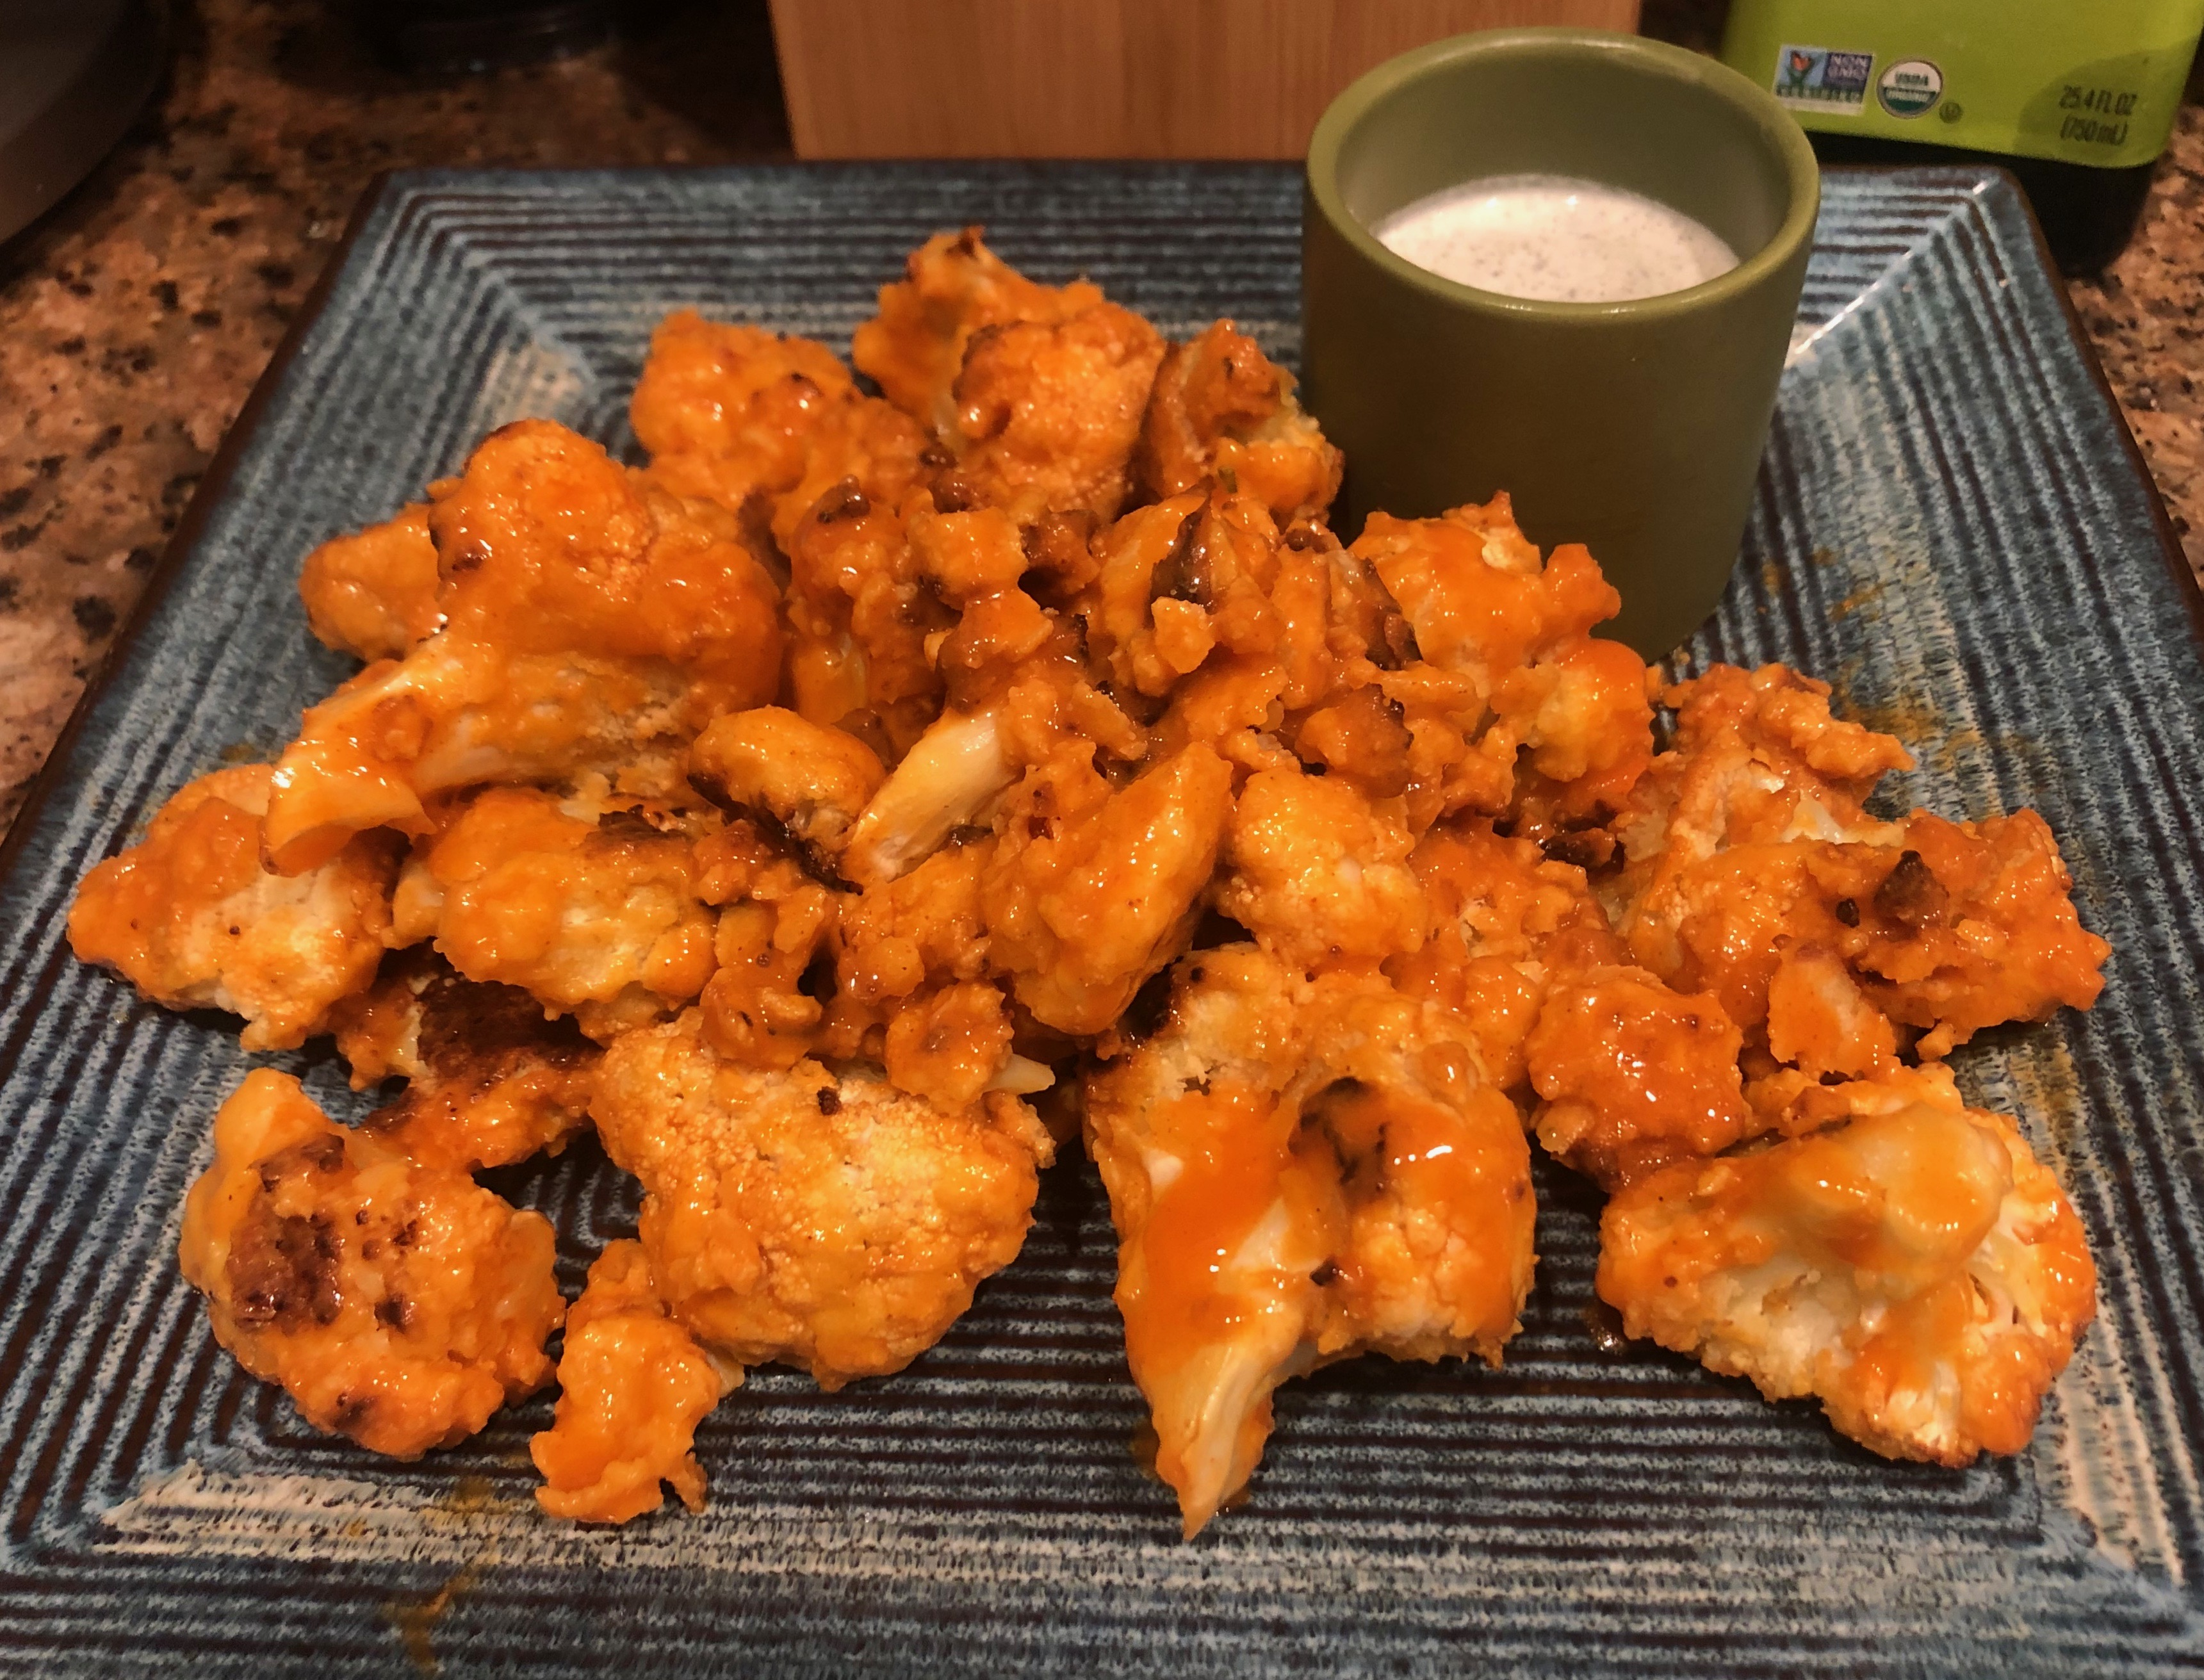
\includegraphics{../food.jpeg}

Ever had the incredible Buffalo Cauliflower from Erewhon? If you
haven't, you MUST! They are probably the first thing that is sold out
everytime we shop\ldots{}THEREFORE I decided to make our
own\ldots{}without the deep fryer! They also use rice flour (which is da
bomb) but for a more keto friendly recipe simply replace with almond
flour ;)

So here you have it- a simple guide to making Vegan, Gluten-free, Keto,
No-Fry Buffalo Cauliflower. Pals and I just so happen to love these on a
rainy days here in LA!

\emph{This way to yum\ldots{}}

\textbf{\textbf{Time}}: 35 Mins. \textbf{\textbf{Yields}}: Roughly two
cups

\textbf{\textbf{Ingredients:}}

\begin{itemize}
\tightlist
\item
  ½ head of Cauliflower
\item
  1 egg
\item
  ½ cup Buffalo sauce (my favorite, ``Red Wings'')
\item
  ½ stick of butter (substitute vegan butter, my favorite ``Miyoko's'')
\item
  1 cup almond flour
\item
  ½ tsp garlic salt
\end{itemize}

\textbf{\textbf{Steps:}}

\textbf{For Cauliflower:}

\begin{enumerate}
\def\labelenumi{\arabic{enumi}.}
\tightlist
\item
  Preheat oven to 450 degrees
\item
  Wash and break cauliflower into pieces, let air dry
\item
  Beat egg with a fork or whisk
\item
  Toss the cauliflower pieces into egg
\item
  Top with Almond flour and garlic salt (we like to use a Ziplock bag to
  toss dry ingredients thoroughly).\\
\item
  Lay on sheet pan with pan liners or foil with a cooking spray. Nothing
  touching to cook evenly
\item
  Bake for 25 minutes or until golden
\end{enumerate}

\textbf{For sauce:}

\begin{enumerate}
\def\labelenumi{\arabic{enumi}.}
\tightlist
\item
  Melt butter/vegan butter
\item
  Add in buffalo sauce
\item
  Whisk or stir thoroughly
\item
  Pour on top of golden cauliflower.
\item
  Serve with hemp-ranch dipping sauce (click here for recipe)
\end{enumerate}

Lol, even the boy said these were \emph{ahhhhmazing!}

\textbf{Besos \& Besos! -Cassarivera}

\chapter{Literature}\label{literature}

Here is a review of existing methods.

\chapter{Methods}\label{methods}

We describe our methods in this chapter.

\chapter{Applications}\label{applications}

Some \emph{significant} applications are demonstrated in this chapter.

\section{Example one}\label{example-one}

\section{Example two}\label{example-two}

\chapter{Final Words}\label{final-words}

We have finished a nice book.

\bibliography{book.bib,packages.bib}


\end{document}
